\documentclass[a4paper]{article}
\usepackage[utf8]{inputenc}
\usepackage[russian,english]{babel}
\usepackage[T2A]{fontenc}
\usepackage[left=10mm, top=20mm, right=18mm, bottom=15mm, footskip=10mm]{geometry}
\usepackage{indentfirst}
\usepackage{amsmath,amssymb}
\usepackage[italicdiff]{physics}
\usepackage{graphicx}
\usepackage{caption}
\usepackage{float}
\usepackage{caption}
\renewcommand{\thefootnote}{\fnsymbol{footnote}}
\usepackage{tablefootnote}
\usepackage{footmisc}
\usepackage{textcomp}
\usepackage{multicol}
\usepackage[parfill]{parskip}
\usepackage{makecell}
\usepackage{array}  
\renewcommand\cellalign{cc} 
\renewcommand\cellgape{\Gape[2pt]} 
\usepackage[utf8]{inputenc}\newcommand{\approxtext}[1]{\ensuremath{\stackrel{\text{#1}}{\approx}}}
\usepackage[colorlinks=true, urlcolor=blue, linkcolor=blue, citecolor=blue]{hyperref}
\graphicspath{{images/}}
\DeclareGraphicsExtensions{.pdf,.png,.jpg}
\usepackage{wrapfig}
\captionsetup{labelformat=empty}
\usepackage{caption}
\captionsetup[figure]{name=Рисунок}
\captionsetup[table]{name=Таблица}
  
\title{\textbf{Отчет о выполненой лабораторной работе 2.2.1}}
\date{}
\author{Котляров Михаил, Б01-402}

\begin{document}

\maketitle
	
	\section{Введение}
	
	\textbf{Цель работы:}: Определение коэффициента диффузии гелия в воздухе\\

	\textbf{Оборудование:} форвакуумный насос; баллон с гелием; манометр; источник питания; магазин сопротивления; мультиметр; установка
	
	\section{Теоретические сведения}
\textit{Диффузией} называют самопроизвольное взаимное проникновение веществ друг в друга, происходящее вследствие хаотичного теплового движения молекул. При перемешивании молекул разного сорта говорят о взаимной (или концентрационной) диффузии.\\
В системе, состоящей из двух компонентов, плотность потока вещества в результате взаимной диффузии описывается законом Фика:
\begin{center}
$\displaystyle j_a = -D\frac{\partial n_a}{\partial x}$, $\displaystyle j_b = -D\frac{\partial n_b}{\partial x}$,
\end{center}
где $D$ -- коэффициент взаимной диффузии компонентов, $j_{ab}$ = плотности потока частиц соответствующего сорта (количество частиц, пересекающих единичную площадку в единицу времени).\\
В данной работе исследуется взаимная диффузия гелия и воздуха. Давление $P$ и температура $T$ в условиях опыта предполагаются неизменными: $P = (n_{He} + n_{\text{В}})k_{\text{Б}}T = const$, где $n_{He}$ и $n_{\text{В}}$ — концентрации (объёмные плотности) диффундирующих газов. Поэтому для любых изменений концентраций справедливо $\Delta n_{\text{В}} = -\Delta n_{He}$. Следовательно, достаточно ограничиться
описанием диффузии одного из компонентов, например гелия $n_{He}$ :
\begin{equation*}
	j_{He} = -D\frac{\partial n_{He}}{\partial x}
	\eqno(1)
\end{equation*}
Проведём теоретическую оценку величины коэффициента взаимной диффузии. В работа мала концентрация гелия, более того, масса атомов гелия много меньше массы молекул, составляющих воздух. При таких условиях перемешивание газов в эксперимента можно рассматривать как диффузию гелия на стационарном форне воздуха. Тогда коэффициент диффузии приблизительно равен
\begin{equation*}
	\displaystyle D = \frac{1}{3}\lambda \bar v,
	\eqno(2)
\end{equation*}
где $\displaystyle \bar v = \sqrt{\frac{8kT}{\pi m}}$ -- средняя тепловая скорость частиц примеси, $\lambda = \frac{1}{n_0\sigma}$ -- длина свободного пробега частиц, $n_0$ --концентрация рассеивающих центров (фона), $\sigma$ -- сечение столкновения частиц примеси с частицами фона. В общем случае необходимо считать $\displaystyle \lambda = \frac{1}{n_\Sigma \sigma}$, где $\displaystyle n_\Sigma = n_{He} + n_{\text{В}} = \frac{P_\Sigma}{kT}$ - полная концентрация частиц. Также  $\displaystyle \bar v$ -- средняя относительная скорость частиц разных сортов. Таким образом, теоретическая оценка предполагает, что коэффициент диффузии не зависит от пропорция элементов, а обратно пропорционален давлению $\displaystyle D \propto \frac{1}{P_\Sigma}$.

\section{Экспериментальная установка и метод измерения}

Рассмотрим подзадачу о диффузии в соединительной
трубке. Предположим сперва, что концентрации примеси
(гелия) на её торцах поддерживаются постоянными и
равными $n_1$ и $n_2$ соответственно. Тогда через некоторое
время в трубке установится стационарный поток частиц, одинаковый в
каждом сечении трубки (в противном случае, если бы поток зависел от x,
частицы бы накапливались в трубке, и процесс перестал бы быть стационарным). Применяя закон Фика в трубке, получим
\begin{equation*}
	j = -D\frac{\partial n}{\partial x} = const.
\end{equation*}
Следовательно, распределение концентрации в трубке n(x) -- линейная функция:
\begin{equation*}
	n(x) = \frac{\Delta n}{L}x,
	\eqno(3)
\end{equation*}
и плотность потока частиц всюду постоянна и равна
\begin{equation*}
	j = -D\frac{\Delta n}{L},
	\eqno(4)
\end{equation*}
где $\Delta n = n_2 - n_1$ -- разность концентраций гелия на концах трубки.\\
Тогда полное число частиц примеси в сосудах равно соответственно $N_1 = n_1V$ и $N_2 = n_2V$. Прозведение плотности потока на площадь сечения трубки S дает количество частиц, пересекающих в единицу времени любое поперечное сечение трубки. Поэтому 
\begin{center}
$\frac{dN_1}{dt} = jS$, $\frac{dN_2}{dt} = -jS$.
\end{center}
Выразим отсюда скорость изменения $\Delta n$. Вычитая из второго равенства
первое и деля результат на объём сосуда $V$ , с учетом (4) получим
\begin{equation*}
	\frac{d(\Delta n)}{dt} = -\frac{\Delta n}{\tau}
	\eqno(5)
\end{equation*}
Интегрируя (5), получаем, что разность концентраций будет убывать по экспоненциальному закону
\begin{equation*}
	\Delta n = \Delta n_0 e^{-\frac{t}{\tau}}
	\eqno(6)
\end{equation*}
где $\tau = \frac{VL}{2DS}$ -- характерное время выравнивания концентраций между сосудами, $\Delta n_0$ -- разность концентраций примеси в сосудах в начальный момент
времени.\\
Для измерения разности концентраций в
установке применяются датчики теплопроводности. Тонкая
платиновая проволочка, протянутая вдоль оси стеклянного цилиндра,
нагревается током. Тепло от проволочки к стенке
цилиндра передаётся главным образом за счёт теплопроводности газа, находящегося внутри цилиндра. При заданной мощности нагревания приращение температуры проволочки и, следовательно, приращение её сопротивления пропорциональны теплопроводности газа. При малой разности $\Delta n$ концентраций в ссудах можно ожидать, что разность теплопроводностей будет изменяться прямо пропорционально $\Delta n$:
\begin{equation*}
	\Delta \kappa = \kappa(n_2) - \kappa(n_1) \approx const \cdot \Delta n.
\end{equation*}
При незначительном различии в составах смесей показания вольтметра, подсоединённого к диагонали моста, будут пропорциональны разности концентраций примеси: $U \propto \Delta \kappa \propto \Delta n$. В процессе диффузии разность концентраций убывает по закону (8), и значит по тому
же закону изменяется напряжение:
\begin{equation*}
	U = U_0 e^{-\frac{t}{\tau}},
	\eqno(7)
\end{equation*}
где $U_0$ — показание гальванометра в начальный момент времени.
\clearpage
\begin{figure}[h!]
    \centering
    \begin{minipage}{0.48\textwidth}
        \centering
        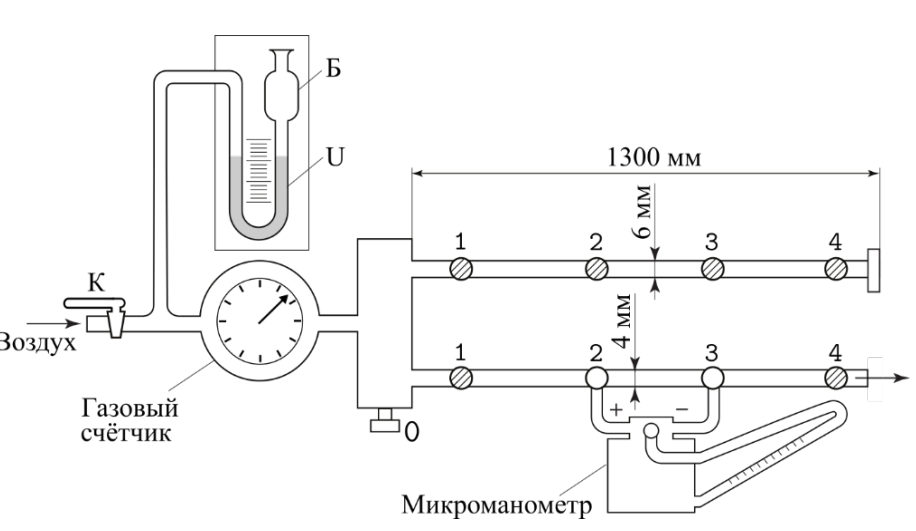
\includegraphics[width=\linewidth]{Pictures/Ustanovka.png}
        \caption{Рис. 1. Экспериментальная установка}
        \label{fig:ustanovka}
    \end{minipage}
    \hfill
    \begin{minipage}{0.48\textwidth}
        \centering
        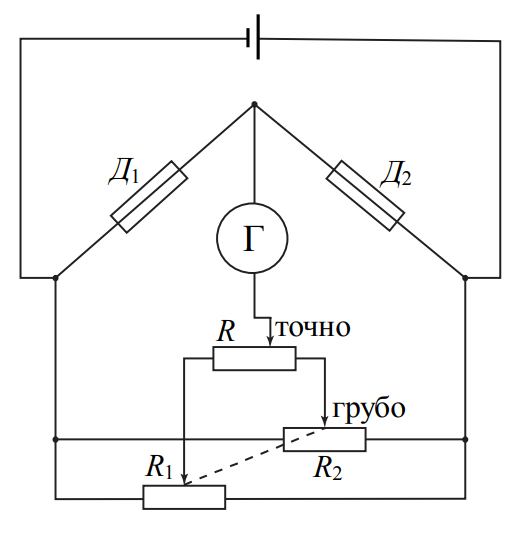
\includegraphics[width=\linewidth]{Pictures/scheme.png}
        \caption{Рис. 2. Электрическая схема установки}
        \label{fig:scheme}
    \end{minipage}
\end{figure}

\section{Приборы и данные}
\begin{itemize}
    \item Вакуумметр образцовый ГОСТ 6521-60, класс точности 0,4.
    \item Форвакуумный насос Адвавак 2, скорость откачки 2 м$^3$/час
	\item Источник постоянного напряжения GW Instek GPS-2303, погрешность 0,5\% + 10 мВ
	\item Цифровой мульиметр Вольтметр универсальный B7-78, погрешность измерения постоянного напряжения 0,0035\% + 0,0005\% диапазона мВ. 
\end{itemize}

\section{Выполнение}
\begin{enumerate}

\item Ход выполнения каждого эксперимента\\
Вначале откачаем до предела воздух из всей установки. Значение на манометре 101,5 делений.  Давление в комнате $756$ торр. По этим данным получаем 1 деление $\approx 7,45$ торр. Запустим в установку воздух до давление $P_1 = 50$ торр. С помощью магазина сопротивлений установик на нити напряжение не более 0,1 мВ. Откачаем весь воздух. Наполним первый сосуд гелием до $0,2P_1$. Откачаем оставшийся в трубках гелий. Накачаем воздух во второй сосуд до давления $1,7P_1$. После этого откроем краны К1 и К2, чтоб давление и температура выровнялись. Закроем краны, зафиксируем получившееся давление в системе, откроем кран К3 и запустим программу, фиксирующую показания вольтметра. Будем ждать, пока напряжение упадет на 30-50\%. Проделаем этот опыт еще 5 раз для разных давлений.\\ 
По полученным данным построим графики зависимости напряжения от времени $U(t)$, а также эту же зависимость в логарифмическом масштабе по оси оридинат.
\clearpage
\begin{figure}[h!]
\centering{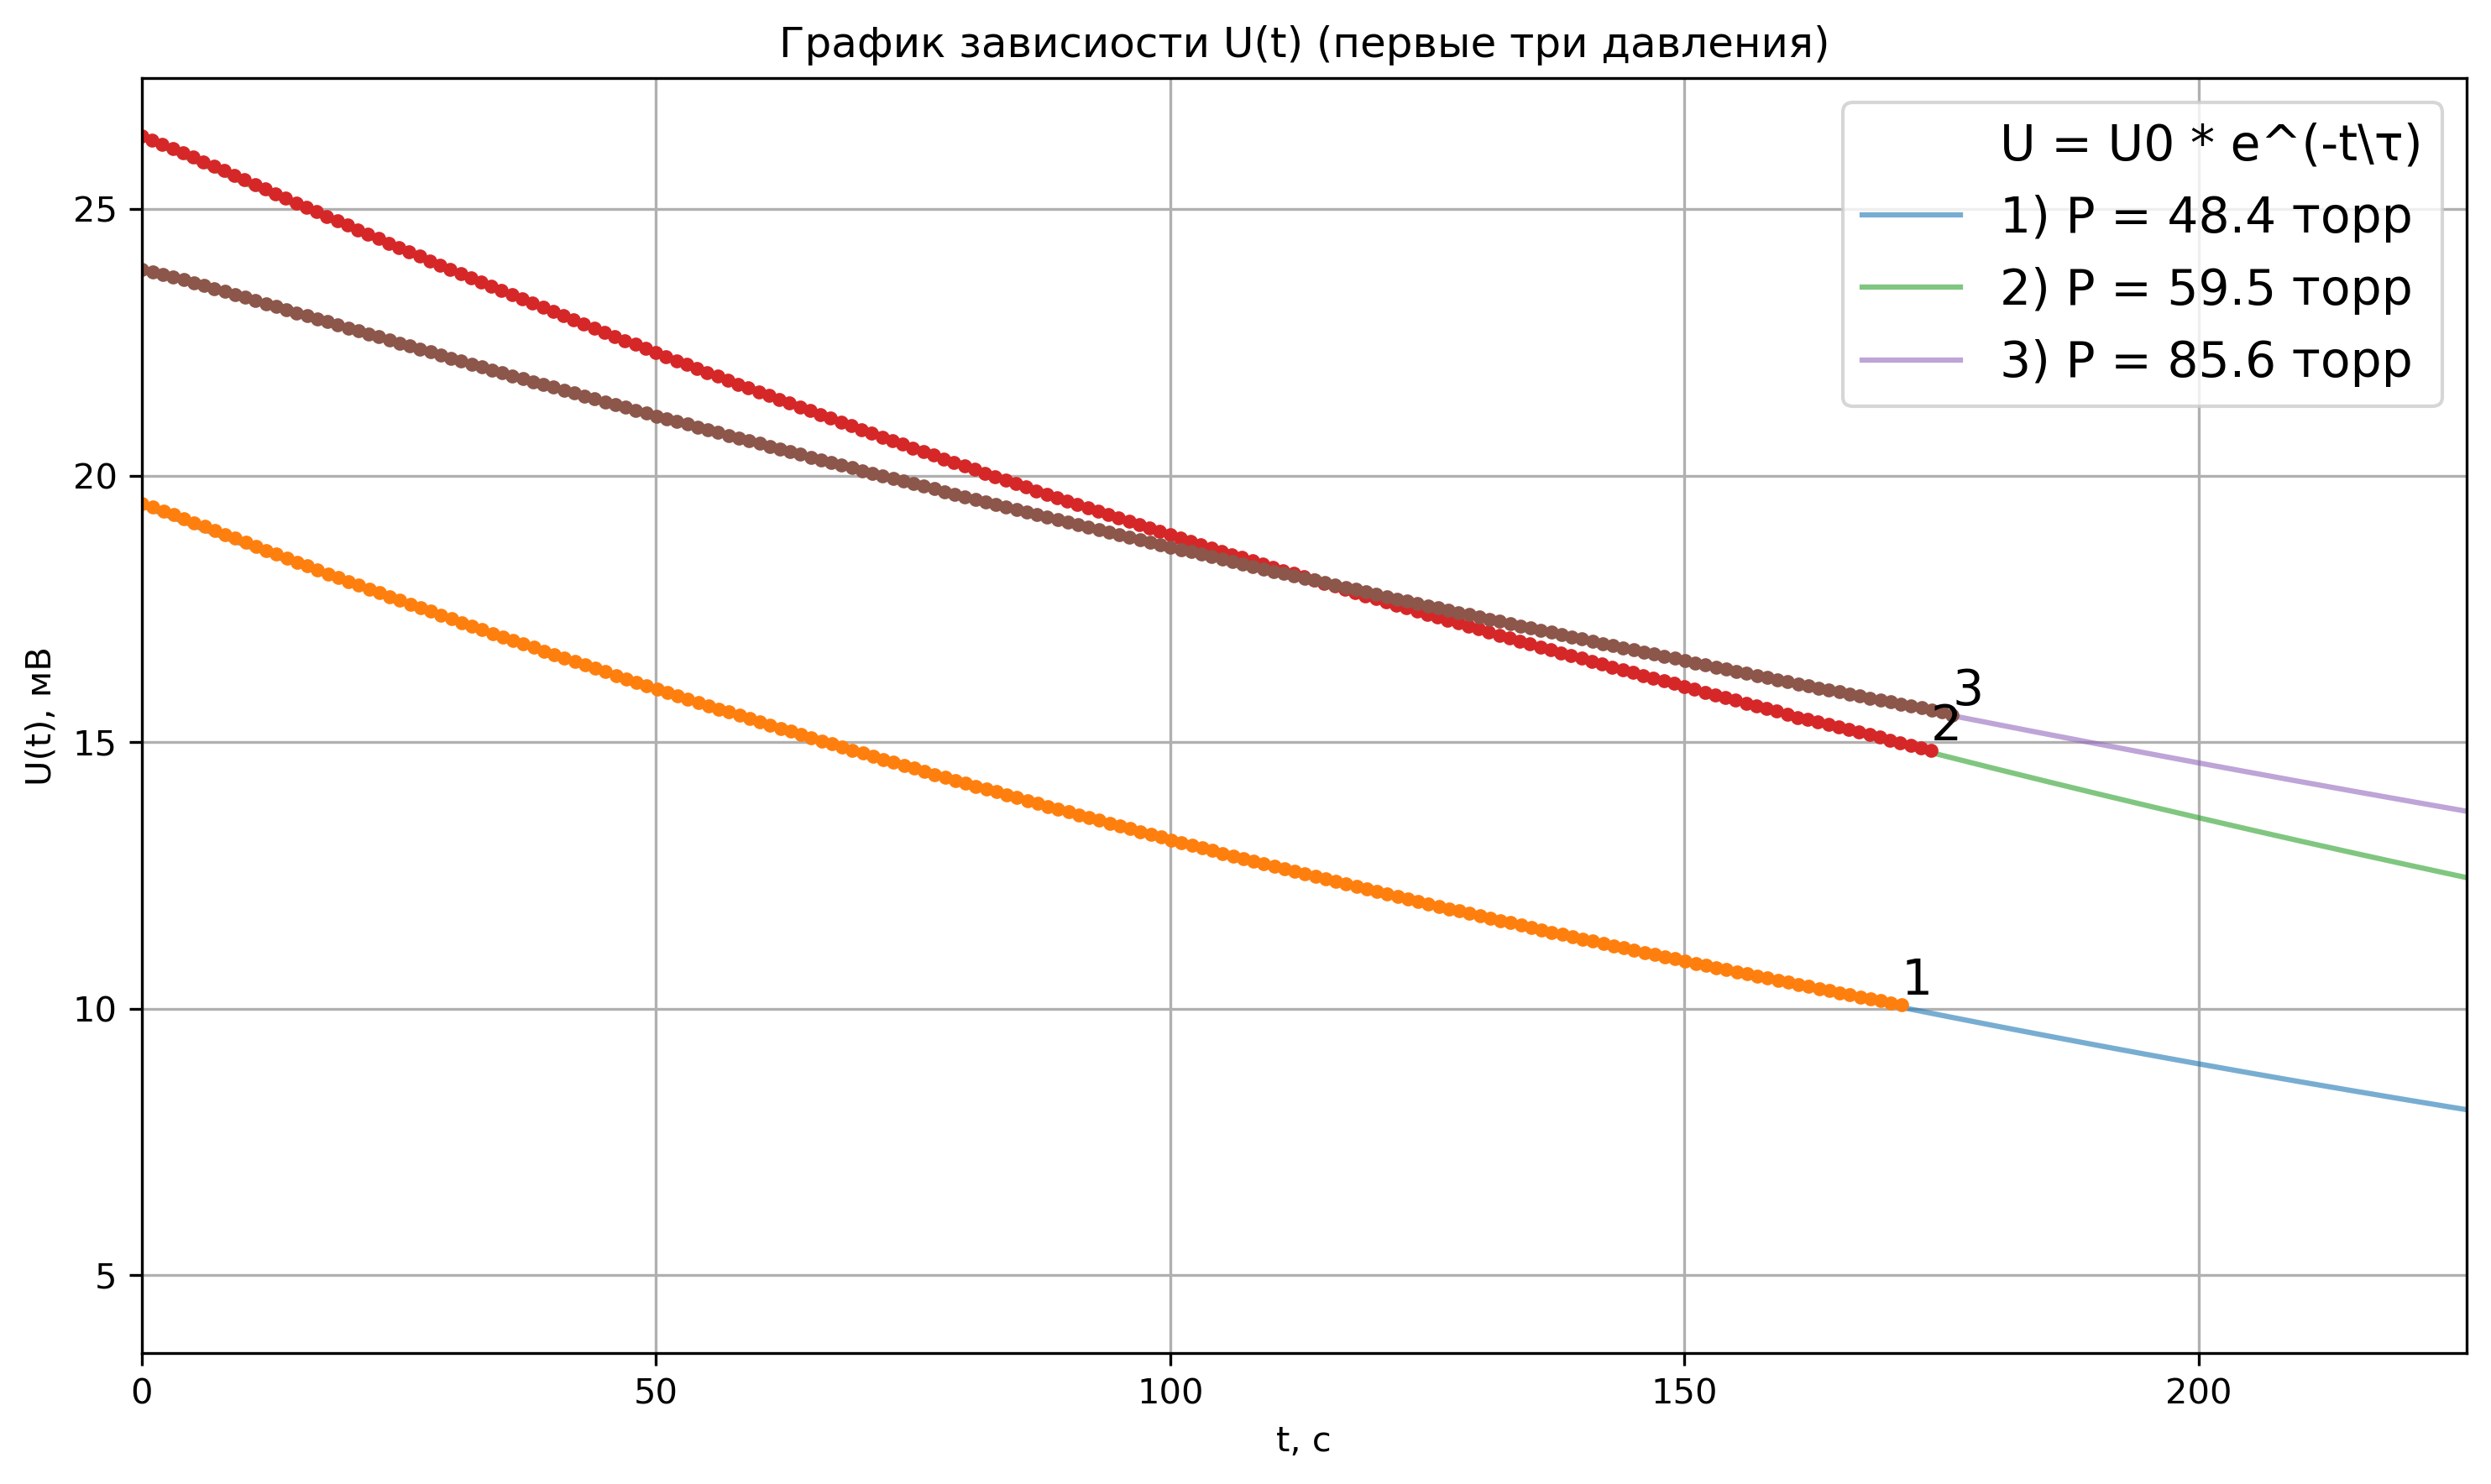
\includegraphics[width=0.8\textwidth]{Graphics/Graph_1.png}}
\caption[]{\label{} Экспоненциальная зависимость напряжения от времени для $P_1$, $P_2$, $P_3$}
\end{figure}
\begin{figure}[h!]
\centering{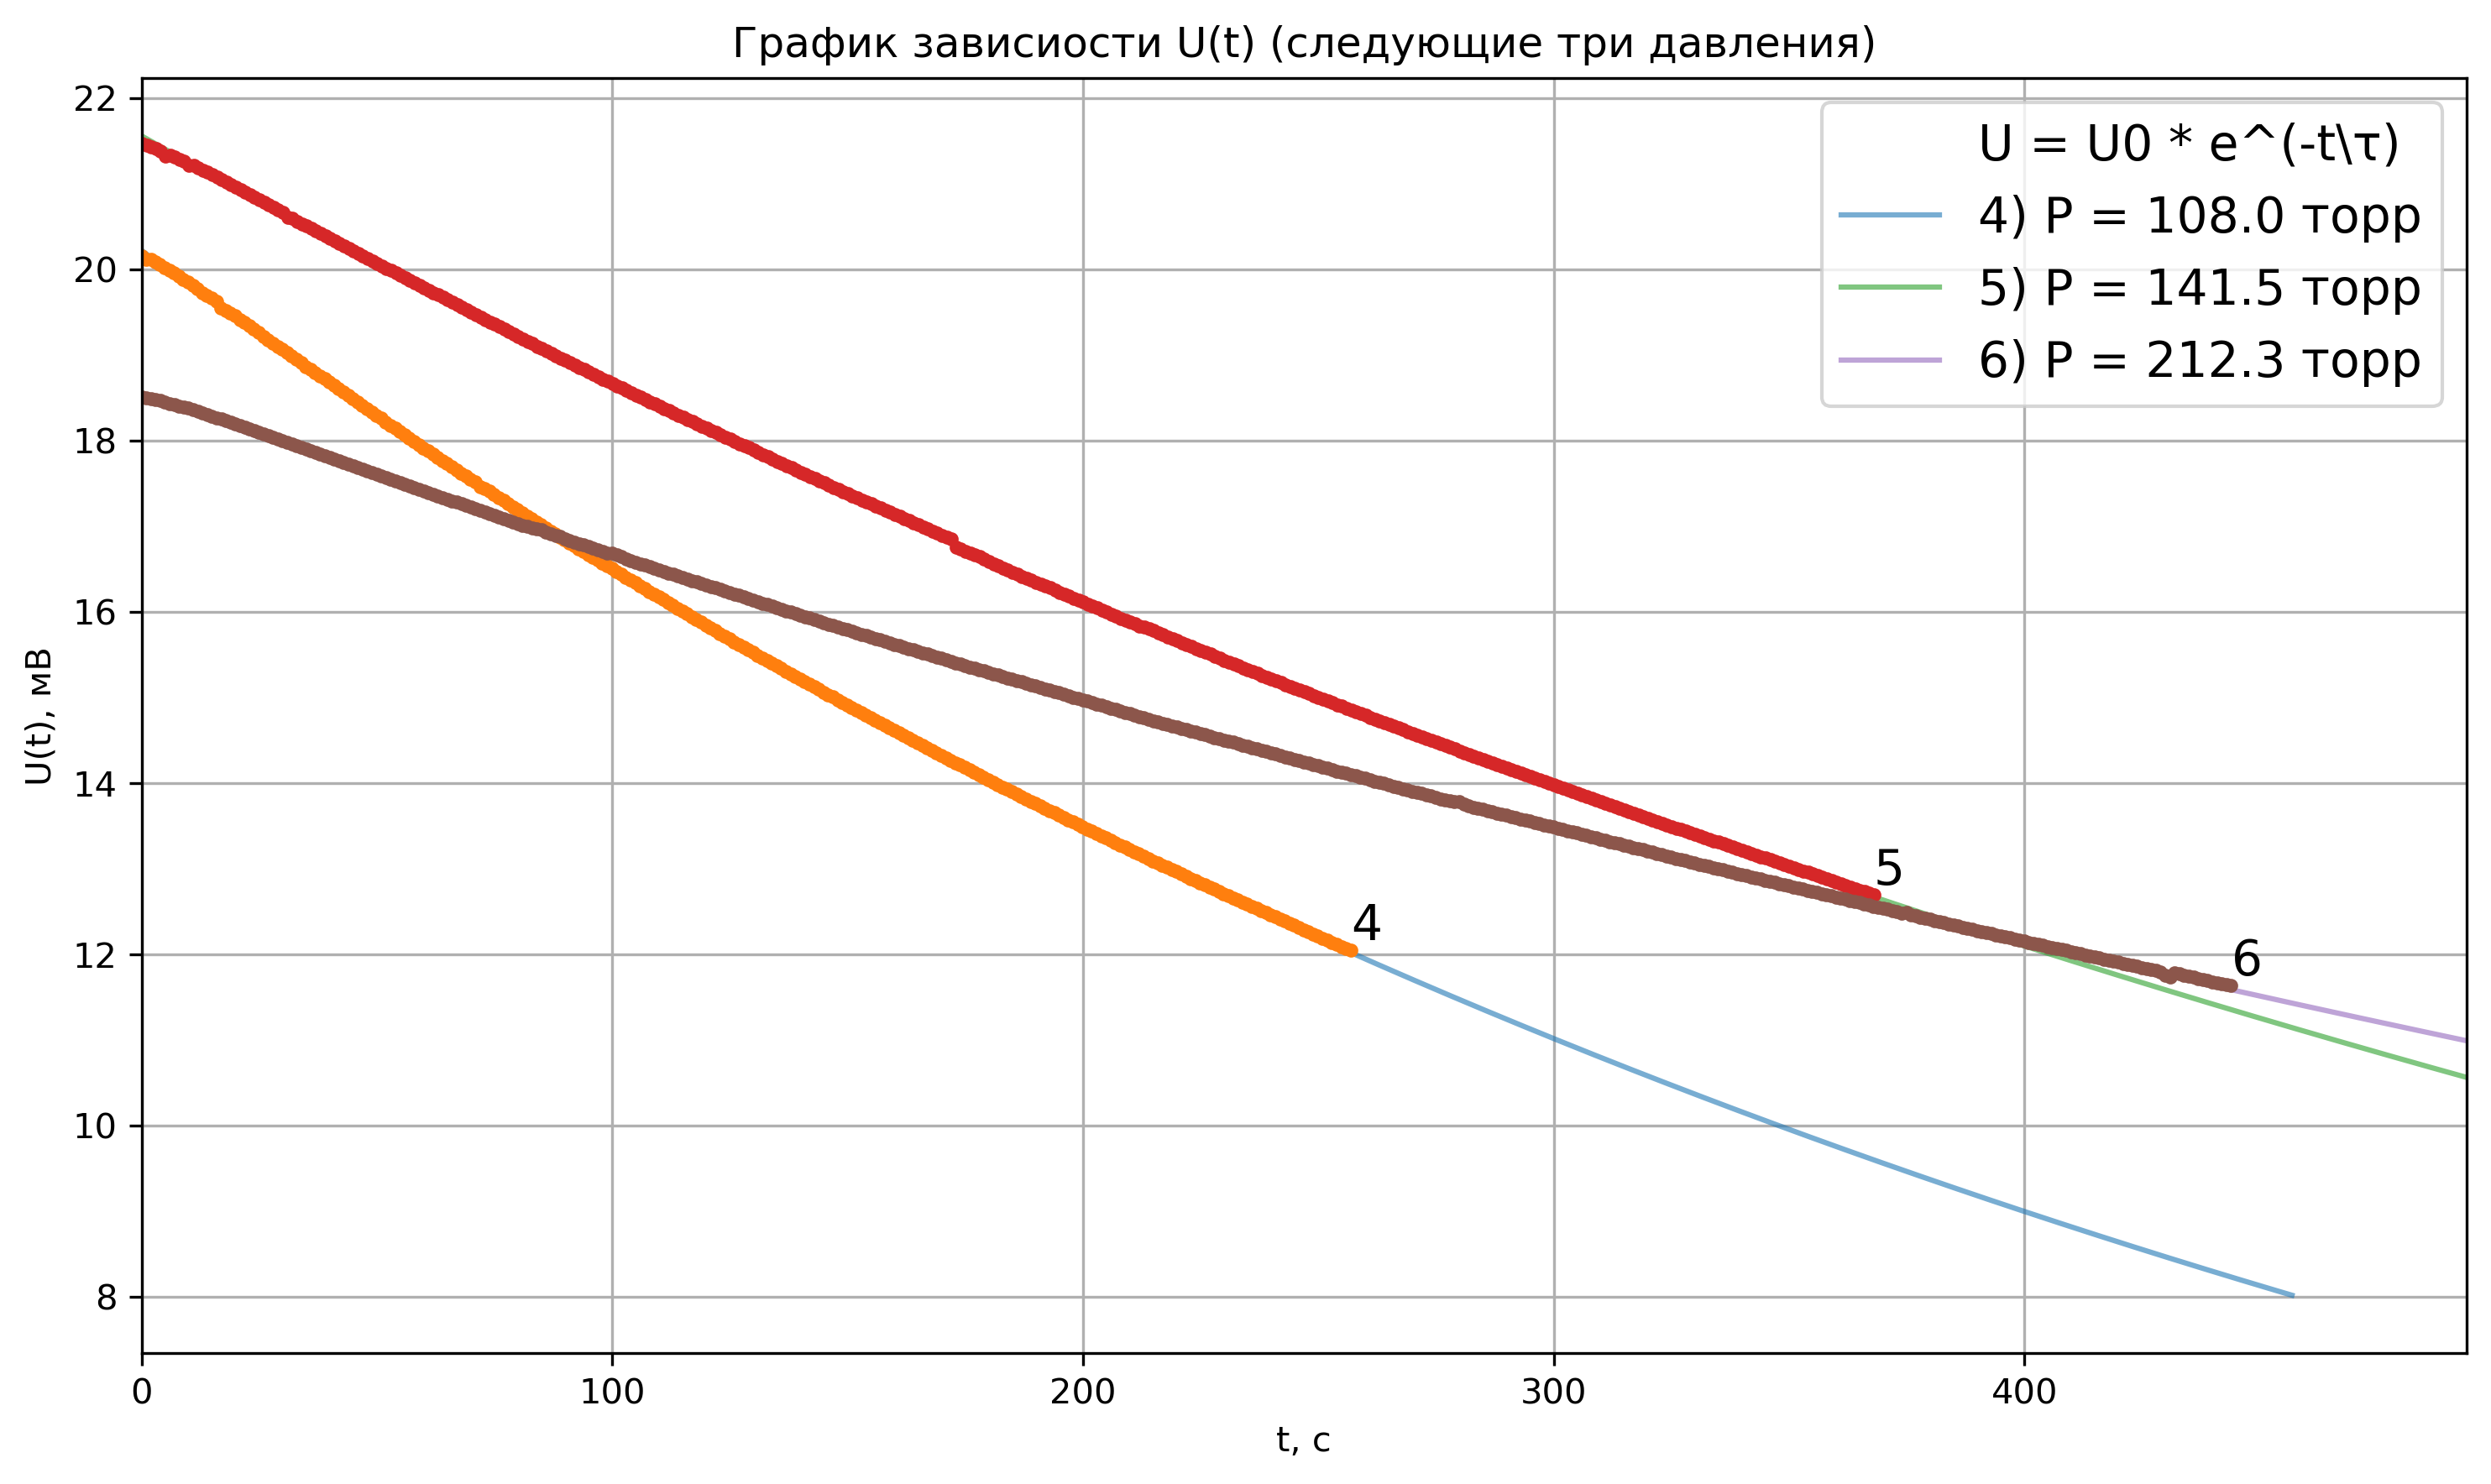
\includegraphics[width=0.8\textwidth]{Graphics/Graph_2.png}}
\caption[]{\label{} Экспоненциальная зависимость напряжения от времени для $P_4$, $P_5$, $P_6$}
\end{figure}
\begin{figure}[h!]
\centering{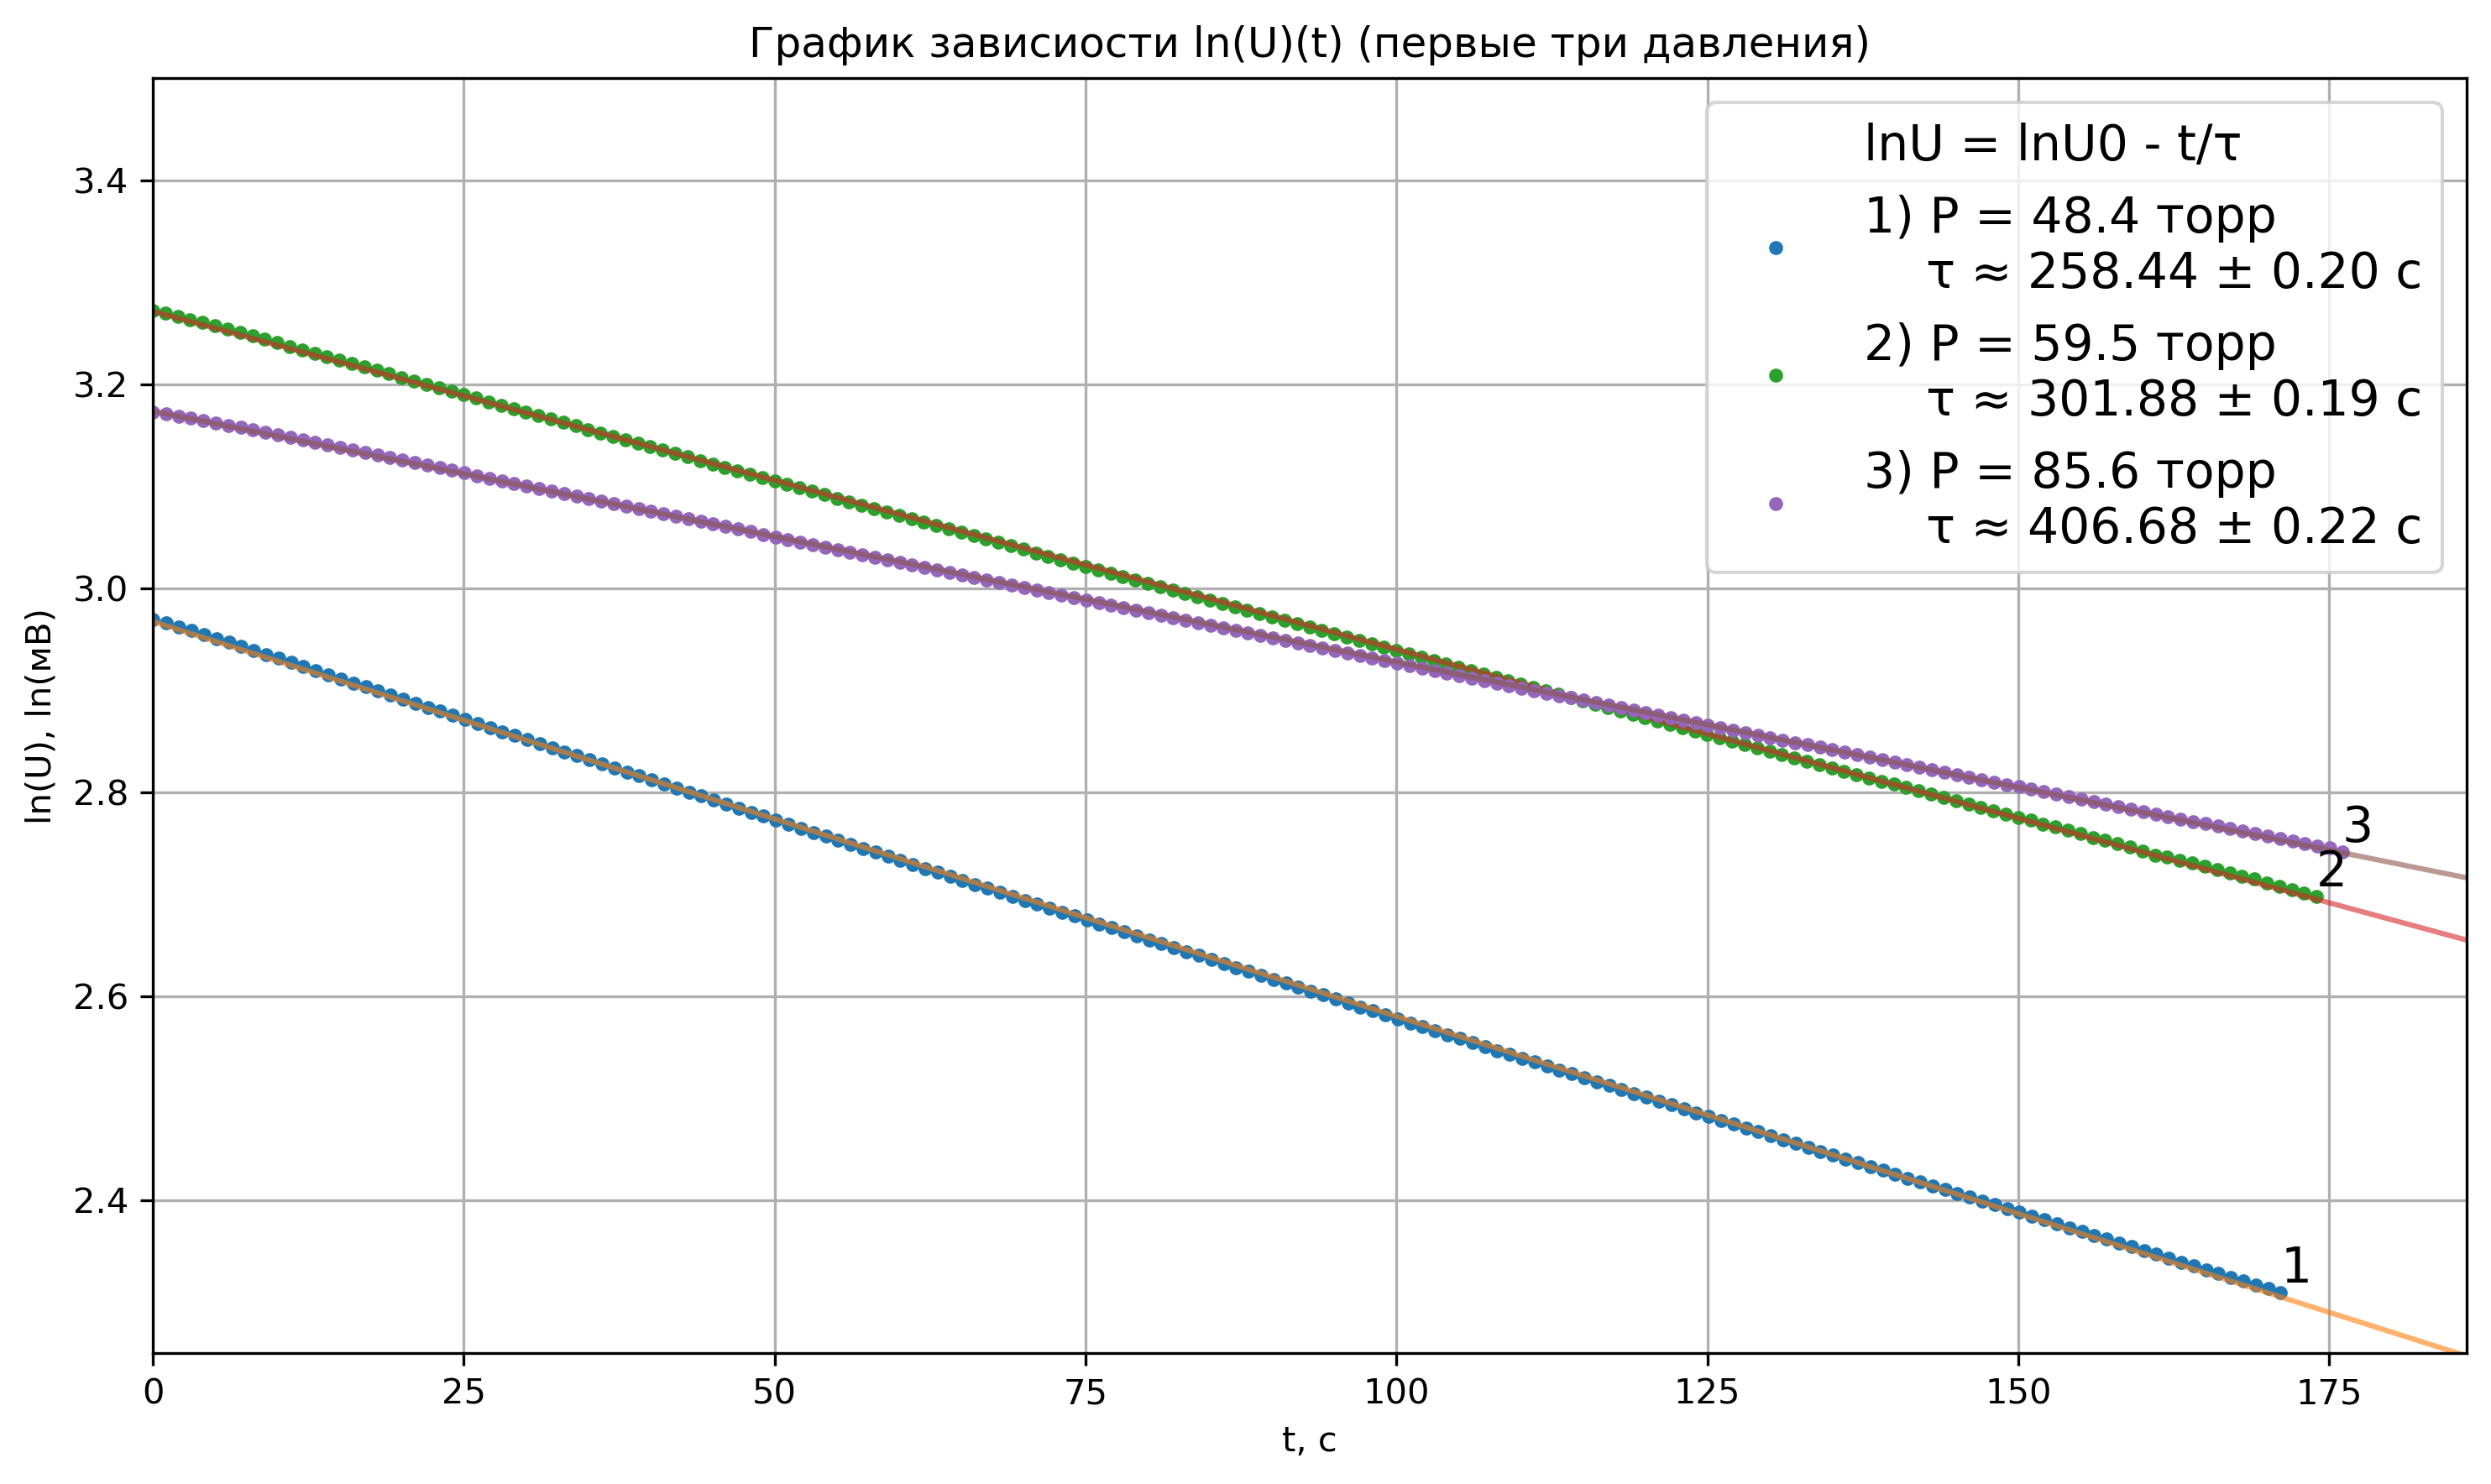
\includegraphics[width=0.8\textwidth]{Graphics/Graph_3.png}}
\caption[]{\label{} Зависимость логарифма напряжения от времени для $P_1$, $P_2$, $P_3$}
\end{figure}
\begin{figure}[h!]
\centering{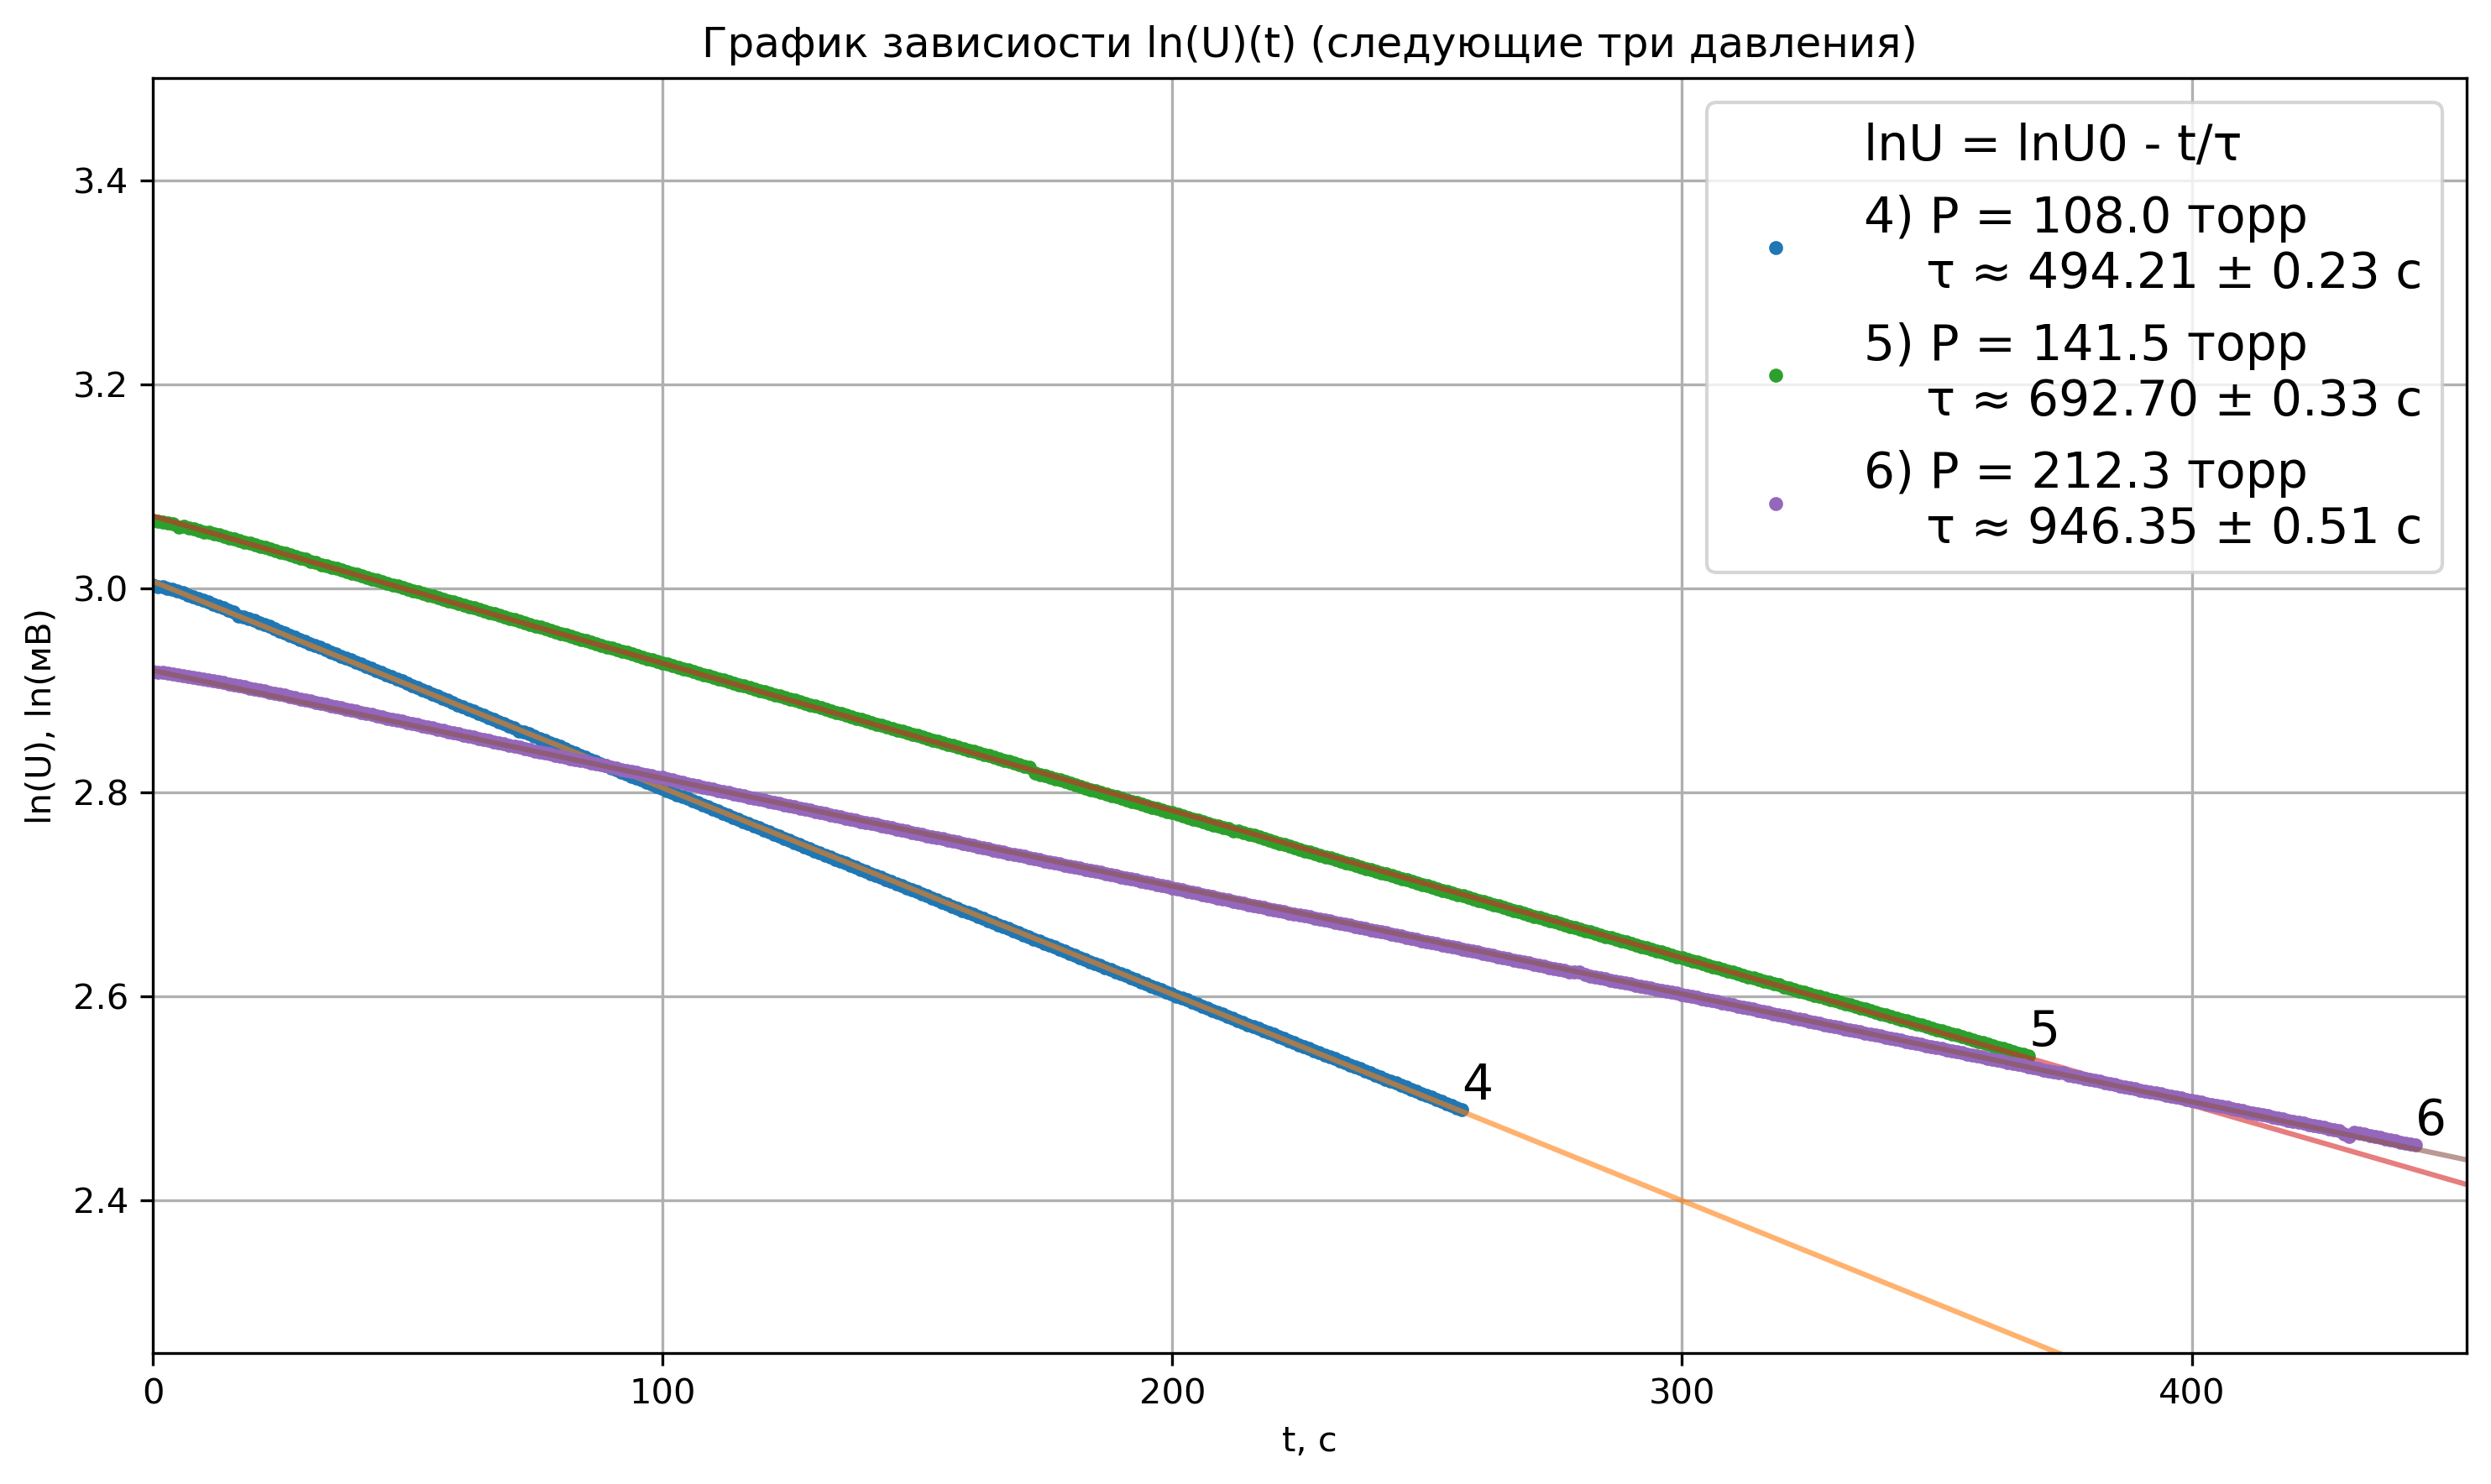
\includegraphics[width=0.8\textwidth]{Graphics/Graph_4.png}}
\caption[]{\label{} Зависимость логарифма напряжения от времени для $P_4$, $P_5$, $P_6$}
\end{figure}
\clearpage

\item По полученным значениям $\tau$ определим коэффициент диффузии для данного давления.

\begin{table}[h!]
    \centering
    \begin{tabular}{|c|c|c|c|c|c|c|}
        \hline
        $P, \text{дел}$ & $P, \text{торр}$ & $\tau, \text{с}$ & $D, \frac{\text{см}^2}{\text{с}}$ & $\sigma_D, \frac{\text{см}^2}{\text{с}}$ & $\varepsilon_D, \%$ \\
        \hline
        $6.5 \pm 0.4$   & $48.4 \pm 3.0$  & $258.44 \pm 0.20$ & 7.31 & 0.19 & 2.63 \\ \hline
        $8.0 \pm 0.4$   & $59.5 \pm 3.0$  & $301.88 \pm 0.19$ & 6.26 & 0.16 & 2.63 \\ \hline
        $11.5 \pm 0.4$  & $85.6 \pm 3.0$  & $406.68 \pm 0.22$ & 4.65 & 0.12 & 2.63 \\ \hline
        $14.5 \pm 0.4$  & $108.0 \pm 3.0$ & $494.21 \pm 0.23$ & 3.82 & 0.10 & 2.63 \\ \hline
        $19.0 \pm 0.4$  & $141.5 \pm 3.0$ & $692.70 \pm 0.33$ & 2.73 & 0.07 & 2.63 \\ \hline
        $28.5 \pm 0.4$  & $212.3 \pm 3.0$ & $946.35 \pm 0.51$ & 2.00 & 0.05 & 2.63 \\
        \hline
    \end{tabular}
    \caption{Таблица 1. Зависимость времени релаксации $\tau$ и диаметра пятна $D$ от давления $P$}
\end{table}

\item По получненным коэффициентам диффузии построим по методу $\chi^2$ зависимость $D(\frac{1}{P})$. Экстраполируя график к атмосферному давлению, оценим соответствующий коэффициент диффузии.

\begin{figure}[h!]
\centering{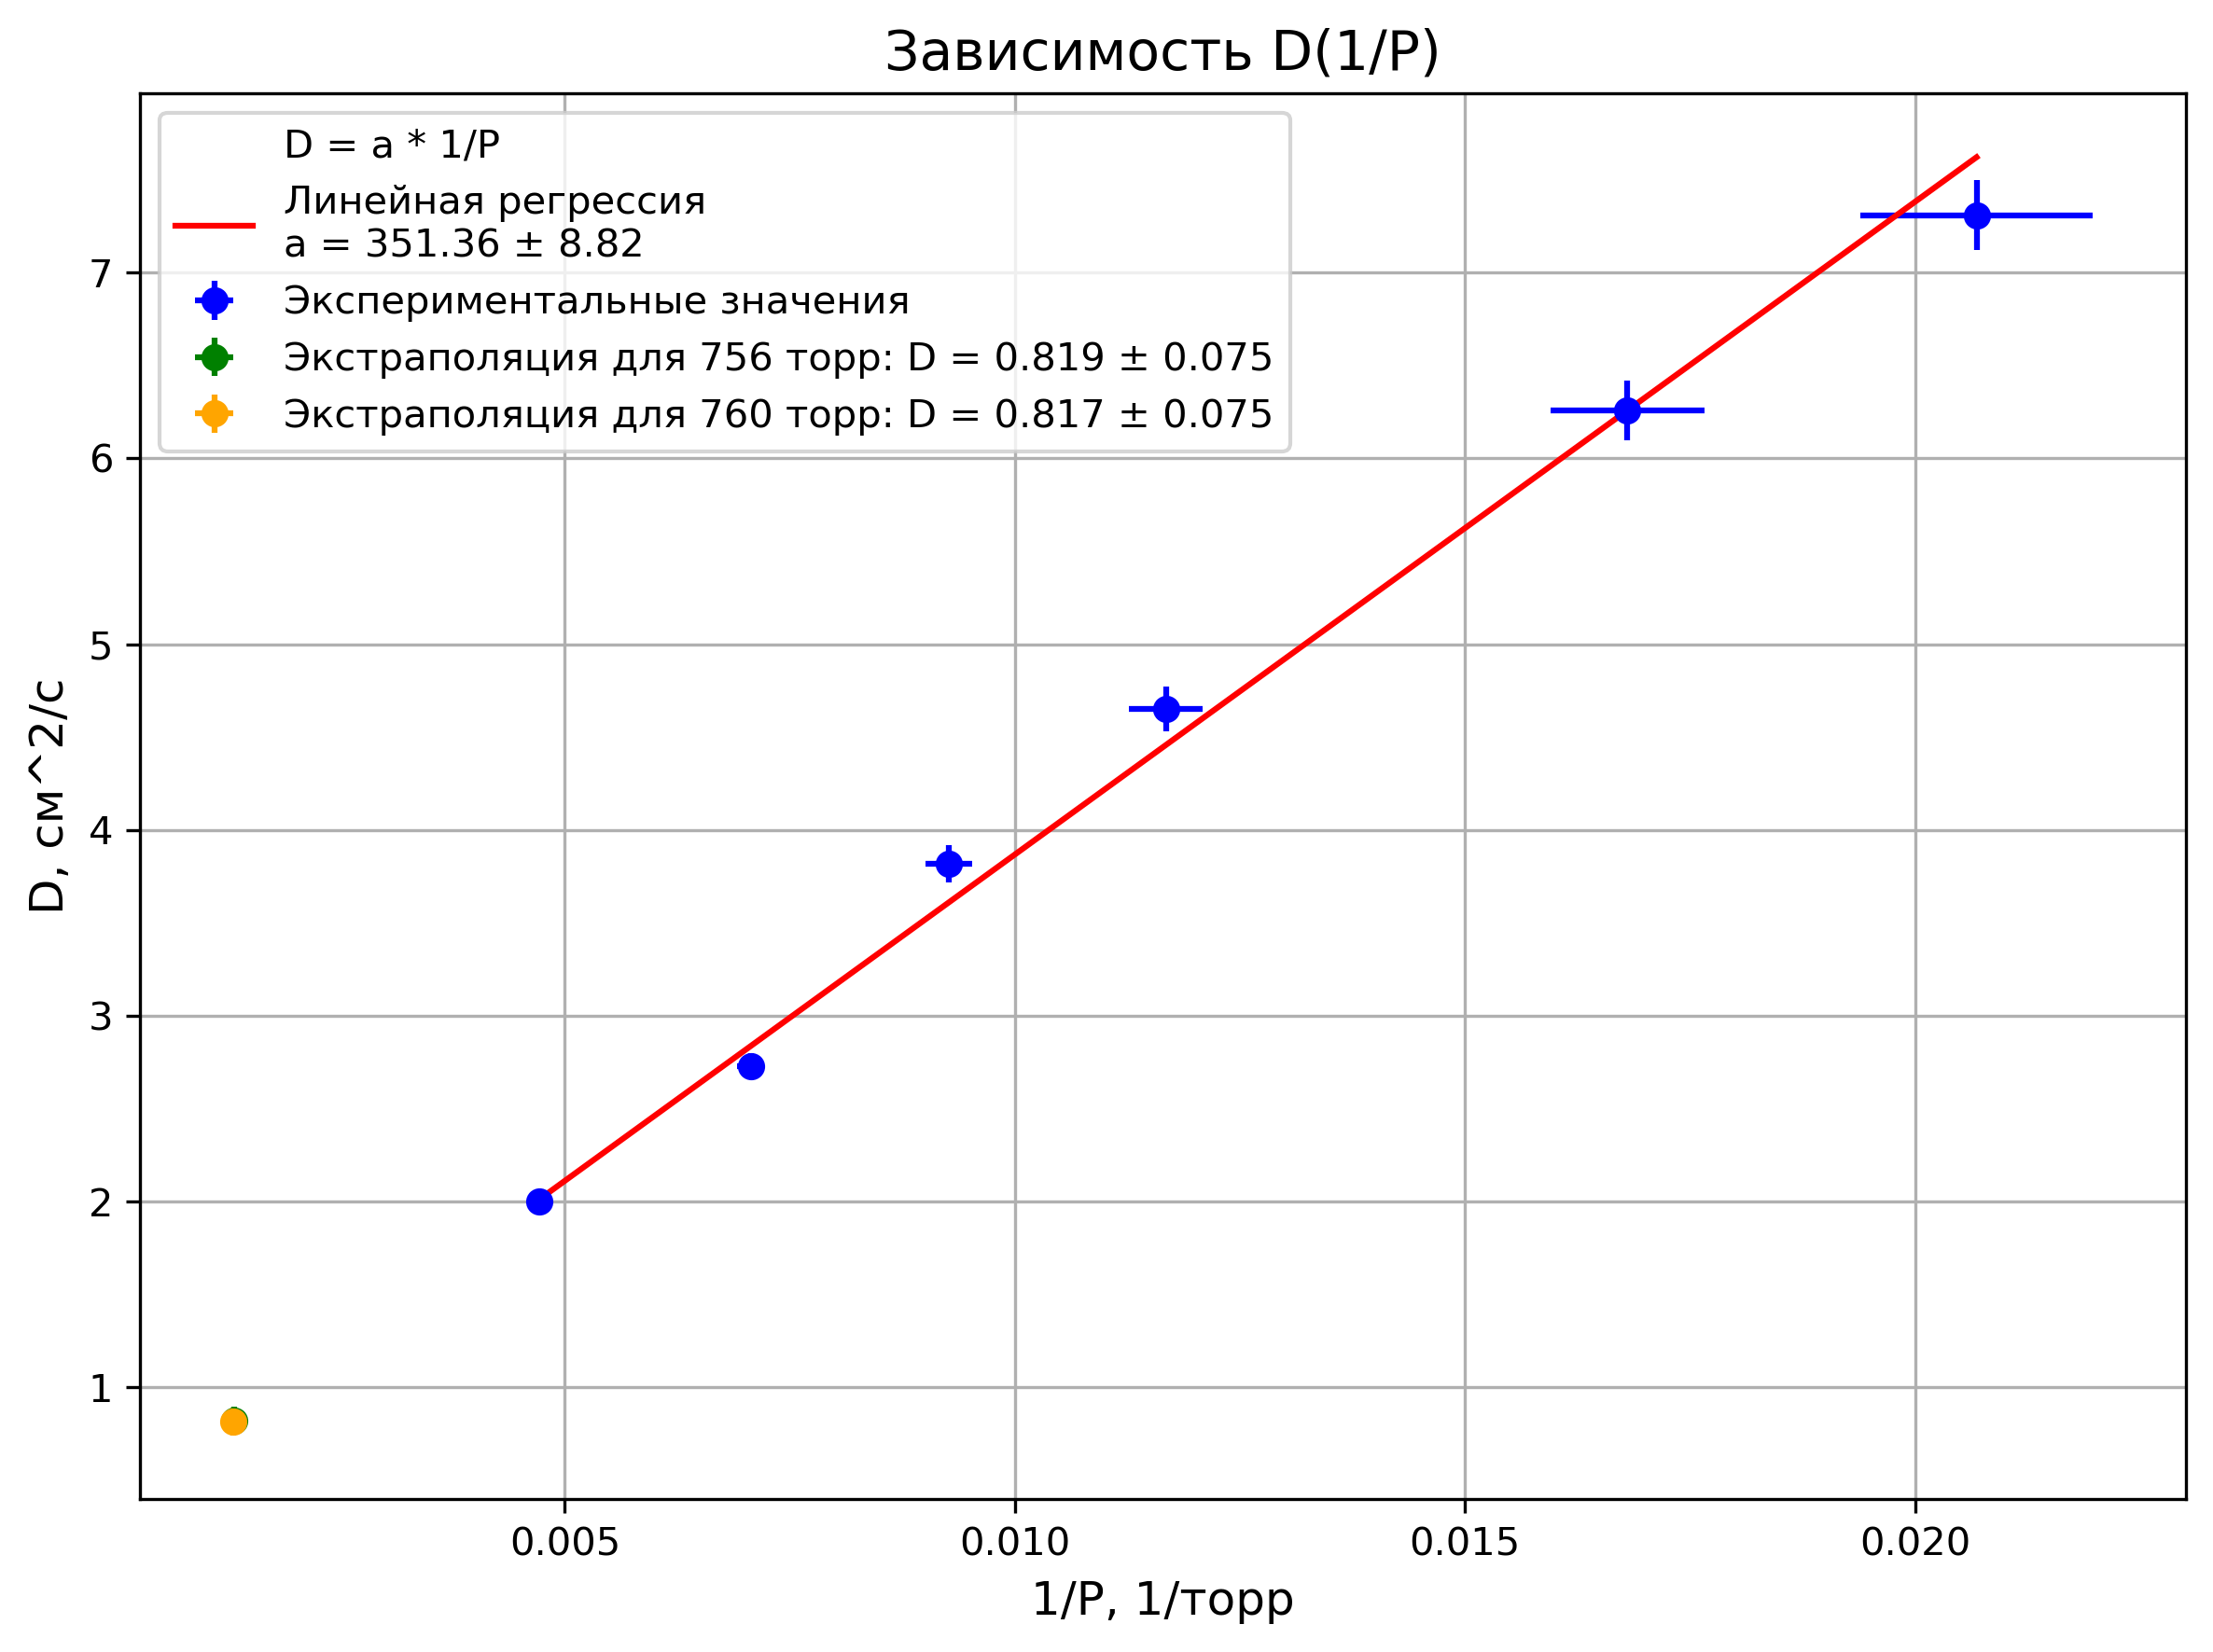
\includegraphics[width=0.75\textwidth]{Graphics/Graph_5.png}}
\caption[]{\label{} Зависимость коэффициента диффузии от обратного давления $D(\frac{1}{P})$}
\end{figure}

Параметры графика: коэффициент наклона $a = 351,36 \pm 8,82$, $\chi^2 = 12.08$, степень свободы $i = 4$, параметр $p = 0.0167$.
Коэффициент диффузии для нашего давления в комнате $D_{756} = 0,820 \pm 0,075 \ \frac{\text{см}^2}{\text{с}}$ ($\varepsilon_{D_{756}} = 9,2 \%$), для нормального атмосферного давления $D_{760} = 0,817 \pm 0,075 \ \frac{\text{см}^2}{\text{с}}$ ($\varepsilon_{D_{756}} = 9,2 \%$).

\item По полученным значениям оценим длину свободного пробега атомов гелия в воздухе $\lambda_{He}$, а также эффективное сечение столкновений атомов гелия с молекулами воздуха $\sigma_{He-\text{возд}}$.\\
Для этого рассчитаем концентрацию молекул $n_0 = \frac{P}{kT}$, $\displaystyle \bar v = \sqrt{\frac{8kT}{\pi m}}$ -- среднюю тепловую скорость частиц примеси.
\begin{equation*}
	n_0^1 = \frac{P_1}{kT_0} = \frac{48,4 \cdot 133,322}{1,38 \cdot 10^{-23} \cdot 298} \approx 1,57 \cdot 10^{24} \text{ м}^{-3}
\end{equation*}
\begin{equation*}
	\sigma_{n_0^1} = n_0^1\frac{\sigma_{P_1}}{P_1} = 1,57 \cdot 10^{24} \frac{3}{48,4} =  9,8 \cdot 10^{22}\text{ м}^{-3}
\end{equation*}
\begin{equation*}
	\varepsilon_{n_0^1} = 6,3 \%
\end{equation*}
\begin{equation*}
\displaystyle \bar v = \sqrt{\frac{8RT}{\pi \mu}} = \sqrt{\frac{8 \cdot 8,31 \cdot 298}{3,1415 \cdot 4 \cdot 10^{-3}}} = 1255,6 \frac{\text{м}}{\text{с}}
\end{equation*}
\begin{equation*}
	\lambda_1 = \frac{3D}{\displaystyle \bar v} = \frac{3 \cdot 7,31 \cdot 10^{-4}}{1255,6} \approx 1747,3 \text{ нм}
\end{equation*}
\begin{equation*}
	\sigma_{\lambda_1} = \lambda_1\varepsilon_{D_1} = 45,9 \text{ нм}
\end{equation*}
\begin{equation*}
	\sigma_{He}^1 = \frac{1}{n_0^1\lambda_1} = \frac{1}{1,57 \cdot 10^{24} \cdot 1747,3 \cdot 10^{-9}} \approx 3,65 \cdot 10^{-19} \text{ м}^2
\end{equation*}
\begin{equation*}
	\Delta_{\sigma_{He}^1} = \sigma_{He}^1 \sqrt{\left(\frac{\sigma_{n_0^1}}{n_0^1}\right)^2 + \left(\frac{\sigma_{\lambda_1}}{\lambda_1}\right)^2} = 1747,3\sqrt{(6,25 \cdot 10^{-2})^2 + (2,63 \cdot 10^{-2})^2} = 2,48 \cdot 10^{-20} \text{ м}^2
\end{equation*}
\begin{equation*}
	\varepsilon_{\sigma_{He}^1} = 6,78 \%
\end{equation*}

\begin{table}[h!]
    \centering
    \begin{tabular}{|c|c|c|c|c|c|c|c|}
        \hline
	$P$, торр & \makecell{$n_0$,\\ $10^{24}$ м$^{-3}$} & \makecell{$\sigma_{n_0}$,\\ $10^{24}$ м$^{-3}$} & $\lambda$, нм & $\sigma_\lambda$, нм & \makecell{$\sigma_{He}$,\\ $10^{-19}$ м$^2$} & \makecell{$\Delta\sigma_{He}$,\\ $10^{-19}$ м$^2$} & $\varepsilon_{\sigma_{He}}$, \% \\
        \hline
        $48.4 \pm 3.0$   & 1.57  & 0.10 & 1747.3 & 45.9 & 3.65 & 0.25 & 6.8 \\ \hline
        $59.5 \pm 3.0$   & 1.93  & 0.10 & 1495.9 & 39.3 & 3.47 & 0.20 & 5.7 \\ \hline
        $85.6 \pm 3.0$   & 2.78  & 0.10 & 1110.4 & 29.2 & 3.24 & 0.14 & 4.4 \\ \hline
        $108.0 \pm 3.0$  & 3.50  & 0.10 & 913.7  & 24.0 & 3.13 & 0.12 & 3.8 \\ \hline
        $141.5 \pm 3.0$  & 4.59  & 0.10 & 651.9  & 17.1 & 3.34 & 0.11 & 3.4 \\ \hline
        $212.3 \pm 3.0$  & 6.88  & 0.10 & 477.2  & 12.5 & 3.04 & 0.09 & 3.0 \\ \hline
        $756.0 \pm 3.0$  & 24.51 & 0.10 & 195.8  & 18.0 & 2.08 & 0.19 & 9.2 \\ \hline
        $760.0 \pm 3.0$  & 24.64 & 0.10 & 195.2  & 18.0 & 2.08 & 0.19 & 9.2 \\
        \hline
    \end{tabular}
    \caption{Таблица 2. Результаты расчёта концентрации $n_0$, длины свободного пробега $\lambda$ и эффективного сечения столкновений $\sigma_{He}$ при различных давлениях $P$}
\end{table}
\renewcommand{\thefootnote}{*} 
Рассчитаем по формулам из теории и табличному значению коэффициента диффузии при атмосферном давлении и температуре $20 ^\circ C$ эти значения. $D_{\text{табл}} = 0{,}697\ \frac{\text{см}^2}{\text{с}}$\footnotemark{}
\footnotetext{Значение данного коэффициента диффузии взято с сайта \url{https://www.engineeringtoolbox.com/air-diffusion-coefficient-gas-mixture-temperature-d_2010.html}}
\renewcommand{\thefootnote}{\arabic{footnote}} 
\begin{equation*}
	\lambda_{\text{табл}} = 166,5 \text{ нм}
\end{equation*}
\begin{equation*}
	\sigma_{\text{табл}} = \frac{1}{n_0^{760}\lambda_{\text{табл}}} = 2,44 \cdot 10^{-19} \text{ м}^2
\end{equation*}

Теперь найдем эффективное сечение столкновений $\sigma_{He}^a$ по коэффициенту ноклона прямой $D(\frac{1}{P})$, поскольку по теории $D = \frac{kT^{\frac{3}{2}}}{3\sigma_{He}}\sqrt{\frac{8R}{\pi \mu}}\frac{1}{P}$. Отсюда $\sigma_{He} = \frac{kT^{\frac{3}{2}}}{3a}\sqrt{\frac{8R}{\pi \mu}}$.
\begin{equation*}
	\sigma_{He}^a = \frac{1}{n_0^{760}\lambda_{\text{табл}}} = 3,68 \cdot 10^{-19} \text{ м}^2
\end{equation*}
\begin{equation*}
	\Delta_{\sigma_{He}^a} = \sigma_{He}^a\frac{\sigma_a}{a} = 3,68 \frac{8,82}{351,36} = 0,09 \cdot 10^{-19} \text{ м}^2
\end{equation*}
\end{enumerate}

\section{Результаты и обсуждения}
\begin{enumerate}
\item По графикам 1-4 отчетливо видно, что процесс диффузии подчиняется закону (6). 
\item Из графика 5 видно, что коэффициент диффузии обратно пропорционален давлению. Об этом говорят значения величин $\frac{\chi^2}{i}$ и $p$.
\item Сравним полученный коэффициент диффузии для атмосферного давления при $25^\circ C$ с табличным для $20^\circ C$.
\begin{table}[h!]
    \centering
    \begin{tabular}{|c|c|c|}
        \hline
        Величина & Эксп. зн. & Табл. зн. \\
        \hline
        $D,\ \frac{\text{см}^2}{\text{с}}$ & $0{,}817$ & $0{,}697$ \\ \hline
        $\sigma_D,\ \frac{\text{см}^2}{\text{с}}$ & $0{,}075$ & $0{,}120$ \\ \hline
        $\varepsilon_D,\ \%$ & $9{,}2$ & $17{,}2$ \\
        \hline
    \end{tabular}
    \caption{Таблица 3. Сравнение экспериментального и табличного значений коэффициента диффузии}
\end{table}
С учетом грубых теоретических приближений, а также погрешностей, результат можно считать приемлимым. 

\item Сравним экспериентальное и высчитанное на основе табличных данных значения эффективного сечения столкновений атомов гелия с молекулами воздуха.
\begin{table}[h!]
    \centering
    \begin{tabular}{|c|c|c|}
        \hline
        Величина & Эксп. зн. & Табл. зн. \\
        \hline
        $\sigma,\ 10^{-19} \text{ м}^2$ & $2{,}079$ & $2{,}437$ \\ \hline
        $\Delta\sigma,\ 10^{-19} \text{ м}^2$ & $0{,}192$ & $0{,}358$ \\ \hline
        $\varepsilon_\sigma,\ \%$ & $9{,}2$ & $14{,}7$ \\
        \hline
    \end{tabular}
    \caption{Таблица 4. Сравнение экспериментального и табличного значений эффективного сечения $\sigma$}
\end{table}

Полученное экспериметнальное значение довольно близко к табличному.
\end{enumerate}

\section{Выводы}
Были проведены 6 серий измерений напряжения от времени для разных давлений. Были построены графики зависимостей $U(t)$, $lnU(t)$. По ним определили коэффициенты диффузии. По полученным данным построили график зависимости $D(\frac{1}{P})$. Экстраполируя график к атмосферному давлению, оценили соответствующий коэффициент диффузии (см таблицу 3). Вычислили длину свободного пробега,  эффективное сечение столкновений атомов гелия с молекулами воздуха для каждого давления. Сравнили со значениями, вычисленными на основе табличного значения коэффициента диффузии.

\end{document}